\PassOptionsToPackage{table}{xcolor}
\documentclass[a4paper,12pt]{beamer}

% -------------------------------------------------
% Theme
% -------------------------------------------------

\usetheme{Berkeley}

% -------------------------------------------------
% Packages
% -------------------------------------------------

\usepackage{tabularx}
\usepackage{array}
\usepackage{graphicx}
\usepackage{listings}
\usepackage{hyperref}
\usepackage{tikz}
\usepackage{pgfplots}
\usepackage[table]{xcolor}
\usepackage[T1]{fontenc}
\usepackage[utf8]{inputenc}

\pgfplotsset{compat=1.18}

\usetikzlibrary{arrows.meta,positioning,shapes.geometric,matrix}

% -------------------------------------------------
% Colors
% -------------------------------------------------

\definecolor{lightgray}{gray}{0.95}

% -------------------------------------------------
% Table of contents styling
% -------------------------------------------------

\setbeamerfont{section in toc}{size=\small}
\setbeamerfont{subsection in toc}{size=\scriptsize}

% -------------------------------------------------
% Listings configuration
% -------------------------------------------------

\lstset{
    language=SQL,
    showspaces=false,
    numbers=left,
    numberstyle=\tiny,
    backgroundcolor=\color{lightgray},
    keywordstyle=\color{blue}\bfseries,
    commentstyle=\color{gray},
    stringstyle=\color{orange},
    basicstyle=\ttfamily\scriptsize,
    breaklines=true,
    literate=
        {é}{{\'e}}1
        {è}{{\`e}}1
        {à}{{\`a}}1
        {ù}{{\`u}}1
        {ç}{{\c{c}}}1
        {ô}{{\^o}}1
        {ê}{{\^e}}1
}

% -------------------------------------------------
% Presentation information
% -------------------------------------------------

\title{Comment minimiser le temps d’exécution de requêtes SQL itérées ?}
\author[Eliott P. \& Antoine BP]{Antoine Bertin--Paillette}
\date{2026}

% -------------------------------------------------
% Footer
% -------------------------------------------------

\setbeamertemplate{footline}{
    \begin{beamercolorbox}[
        wd=\paperwidth,
        ht=2.5ex,
        dp=1ex
    ]{author in head/foot}
        \usebeamerfont{author in head/foot}
        \hspace*{2ex}
        \insertshortauthor
        \hfill
        \inserttitle
        \hfill
        \insertdate
        \hfill
        \insertframenumber/\inserttotalframenumber
        \hspace*{2ex}
    \end{beamercolorbox}
}

% Remove navigation symbols
\setbeamertemplate{navigation symbols}{}

% -------------------------------------------------
% Compact top header
% -------------------------------------------------

\setbeamertemplate{headline}{
    \leavevmode
    \begin{beamercolorbox}[
        wd=\paperwidth,
        ht=1.5ex,
        dp=0.6ex
    ]{section in head/foot}
    \end{beamercolorbox}
}

% -------------------------------------------------
% Sidebar configuration
% -------------------------------------------------

% Narrower sidebar
\setbeamersize{sidebar width left=2.4cm}

% Display sections + subsections
\setbeamertemplate{sidebar left}{
    \vspace{0.5em}
    \insertverticalnavigation{\beamersidebarwidth}
}

% Smaller fonts (prevents overflow)
\setbeamerfont{section in sidebar}{size=\scriptsize}
\setbeamerfont{subsection in sidebar}{size=\tiny}

% Brighter colors
\setbeamercolor{section in sidebar}{
    fg=white,
    bg=blue!75
}

\setbeamercolor{section in sidebar shaded}{
    fg=white!75
}

\setbeamercolor{subsection in sidebar}{
    fg=white!90,
    bg=blue!25
}

\setbeamercolor{subsection in sidebar shaded}{
    fg=white!65
}

% -------------------------------------------------
% Automatic section TOC slide
% -------------------------------------------------



\begin{document}

\begin{frame}
    \titlepage\
\end{frame}
\begin{frame}
    \frametitle{Sommaire}
    \tableofcontents[hideallsubsections]
\end{frame}

\section{But du TIPE}

\subsection{Description du jeux de données}

\begin{frame}
    \frametitle{Description du jeux de données}

  \begin{block}{Nous avons choisi de travailler sur les données de wikipedia}
    \begin{itemize}
        \item  Des données de pages: titre, contenu, thème, modifications
        \item  Des données d'utilisateur: nom, date d'inscription, nombre de modification
        \item  Des révisions de pages
    \end{itemize}
    \end{block}


\end{frame}



\begin{frame}{Exemple du jeu de données Wikipédia}

\scriptsize

\begin{block}{Extrait du jeu de données}
\centering
\begin{tabular}{r c l r}
\textbf{id} & \textbf{ns} & \textbf{title} & \textbf{revision\_id} \\
\hline
3  & 0 & Antoine Meillet & 230038204 \\
10 & 0 & Algorithmique & 226806957 \\
15 & 0 & Autriche & 229636050 \\
18 & 0 & Arsène Lupin & 230120442 \\
23 & 0 & Afghanistan & 230208941 \\
27 & 0 & Ada (langage) & 226996025 \\
35 & 0 & Alpes-Maritimes & 229772008 \\
42 & 0 & Argentine & 230240365 \\
44 & 0 & Akira Kurosawa & 228584801 \\
\end{tabular}
\end{block}

\vspace{0.2cm}

\begin{block}{Exemple de données de révision}
\centering
\begin{tabular}{r r r r}
\textbf{id} & \textbf{parent\_id} &
\textbf{timestamp} & \textbf{contributor\_id} \\
\hline
230038204 & 226458976 & 1761327915 & 316223 \\
226672222 & 216521656 & 1750499141 & 5256901 \\
228034381 & 228034155 & 1754898945 & 1430140 \\
\end{tabular}
\end{block}

\end{frame}

\subsection{Que faire des résultats ?}

\begin{frame}{Que faire des résultats ?}
    \begin{columns}[T]
        \column{0.48\textwidth}
        \begin{block}{Requêtes typiques}
            \begin{itemize}
                \item Classement des utilisateurs les plus actifs par catégorie
                \item Utilisateurs experts d'une catégorie
                \item Pages les plus modifiées par catégorie
            \end{itemize}
        \end{block}

        \column{0.48\textwidth}
        \begin{block}{Utilisations des résultats}
            \begin{itemize}
                \item Récolter et afficher des statistiques utilisateur
                \item Trier, comparer, sélectionner
                \item Recommander / rechercher des pages selon des critères
            \end{itemize}
        \end{block}
    \end{columns}
\end{frame}

\begin{frame}[fragile]{Exemples de requêtes SQL}

\scriptsize

\begin{block}{1. Classement des utilisateurs les plus actifs par catégorie}
\begin{lstlisting}
SELECT c.category_name,
       u.username,
       COUNT(*) AS edits
FROM revisions r
JOIN users AS u ON r.user_id = u.user_id
JOIN pages AS p ON r.page_id = p.page_id
JOIN categories c ON p.category_id = c.category_id
GROUP BY c.category_name, u.username
ORDER BY c.category_name, edits DESC;
\end{lstlisting}
\end{block}

\vspace{-0.2cm}

\begin{block}{2. Pages les plus modifiées par catégorie}
\begin{lstlisting}
SELECT c.category_name,
       p.title,
       COUNT(*) AS revisions
FROM revisions r
JOIN pages AS p ON r.page_id = p.page_id
JOIN categories AS c ON p.category_id = c.category_id
GROUP BY c.category_name, p.title
ORDER BY revisions DESC;
\end{lstlisting}
\end{block}

\end{frame}

\section{Réalisation}

\subsection{Ce qui est prévu}
\begin{frame}
    \frametitle{Ce qui est prévu}
	\begin{figure}[h]
		\centering
		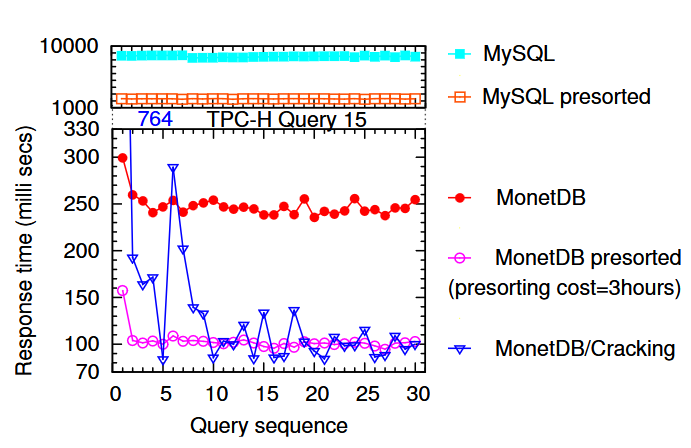
\includegraphics[width=250pt]{ressource/perf_comparaison.png}
    \caption{Notre objectif est de comparer avec ce genre de graphique notre implémentation et ce qui a déjà été fait.}
	\end{figure}
\end{frame}

\subsection{Ce qui a été fait}
\begin{frame}
    \frametitle{Ce qui a été fait}
 \begin{block}{Ce que nous avons implémenté}
    \begin{itemize}
        \item  Une BDD fonctionnelle pour la plupart des requêtes
        \item  Des optimisations du plan
        \item  Tester un grand nombre de requêtes et enregistrer les temps
        \item  Les optimisations mémoire
        \item  Comparer avec des implémentation existentes
        \item  Améliorer et optimiser certaines parties imparfaite de l'implémentation
    \end{itemize}
    \end{block}
\end{frame}



\section{Optimisations mémoire}

\subsection{Paradigme ligne VS colonne}

\begin{frame}{Paradigme ligne VS colonne}
    \begin{columns}[T]
        \column{0.48\textwidth}
        \begin{block}{Orientée lignes}
            \footnotesize
            \begin{itemize}
                \item Stockage par enregistrement complet
                \item Efficace pour \texttt{SELECT *}
                \item Lit des colonnes inutiles pour les agrégations
            \end{itemize}
        \end{block}
        \vspace{0.2cm}
        \begin{exampleblock}{Exemple (PostgreSQL, MySQL)}
            \centering\scriptsize
            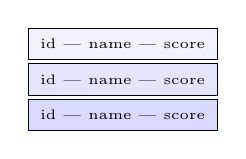
\begin{tikzpicture}
                \draw[fill=blue!15] (0,0) rectangle (2.4,0.4)
                    node[midway]{\tiny id | name | score};
                \draw[fill=blue!10] (0,0.45) rectangle (2.4,0.85)
                    node[midway]{\tiny id | name | score};
                \draw[fill=blue!5]  (0,0.9)  rectangle (2.4,1.3)
                    node[midway]{\tiny id | name | score};
            \end{tikzpicture}
        \end{exampleblock}

        \column{0.48\textwidth}
        \begin{block}{Orientée colonnes}
            \footnotesize
            \begin{itemize}
                \item Stockage par attribut
                \item Meilleure compression
                \item Très efficace pour les agrégations analytiques
            \end{itemize}
        \end{block}
        \vspace{0.2cm}
        \begin{exampleblock}{Exemple (MonetDB, C-Store)}
            \centering\scriptsize
            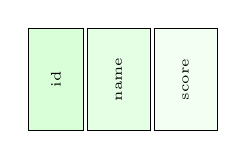
\begin{tikzpicture}
                \draw[fill=green!15] (0,0)    rectangle (0.7,1.3)
                    node[midway,rotate=90]{\tiny id};
                \draw[fill=green!10] (0.75,0) rectangle (1.55,1.3)
                    node[midway,rotate=90]{\tiny name};
                \draw[fill=green!5]  (1.6,0)  rectangle (2.4,1.3)
                    node[midway,rotate=90]{\tiny score};
            \end{tikzpicture}
        \end{exampleblock}
    \end{columns}
    \vfill
    {\tiny Source : Abadi et al., \textit{Column-Stores vs. Row-Stores} (SIGMOD 2008)}
\end{frame}

\begin{frame}{Bases orientées colonnes vs orientées lignes}
\small
\begin{block}{Temps d'exécution normalisés (base ligne = 100)}
\centering\tiny Requêtes analytiques typiques : \texttt{SUM}, \texttt{GROUP BY}, jointures.
\end{block}
\vspace{-0.15cm}
\begin{center}
\begin{tikzpicture}
\begin{axis}[
    width=0.90\textwidth,
    height=0.64\textheight,
    ybar,
    bar width=7pt,
    ymin=0, ymax=267,
    ylabel={Temps relatif (base ligne = 100)},
    symbolic x coords={
        Lecture\\3 colonnes,
        Agrégation\\SUM,
        GROUP BY,
        Jointure
    },
    xtick=data,
    xticklabel style={align=center, font=\scriptsize},
    legend style={at={(0.5,1.02)}, anchor=south,
                  legend columns=3, font=\scriptsize},
    nodes near coords,
    nodes near coords style={font=\tiny},
    enlarge x limits=0.2,
    grid=major
]
\addplot coordinates {
    (Lecture\\3 colonnes,100)(Agrégation\\SUM,100)
    (GROUP BY,100)(Jointure,100)};
\addplot coordinates {
    (Lecture\\3 colonnes,6)(Agrégation\\SUM,12)
    (GROUP BY,10)(Jointure,15)};
\addplot coordinates {
    (Lecture\\3 colonnes,155)(Agrégation\\SUM,127)
    (GROUP BY,238)(Jointure,226)};
\legend{Orientée lignes, Orientée colonnes, Nos performances}
\end{axis}
\end{tikzpicture}
\end{center}
\vspace{-0.15cm}
{\tiny
Sources : Abadi et al., \textit{Column-Stores vs. Row-Stores} (SIGMOD 2008) ;
\textit{The Design and Implementation of Modern Column-Oriented Database Systems} (2013).
}
\end{frame}

\subsection{Indexation des données}

\begin{frame}{Indexation des données — exemple Wikipédia}
\small

\begin{columns}[T]

% ── Colonne gauche : index ────────────────────────
\column{0.38\textwidth}
\centering
{\scriptsize\textbf{Index sur \texttt{page\_id}}}\\[4pt]

\scriptsize
\setlength{\tabcolsep}{5pt}
\begin{tabular}{r l}
  \textbf{page\_id} & \textbf{pointeur} \\
  \hline
  3  & $\rightarrow$ ligne 1 \\
  10 & $\rightarrow$ ligne 2 \\
  \rowcolor{blue!10}
  15 & $\rightarrow$ ligne 3 \\
  \rowcolor{blue!10}
  18 & $\rightarrow$ ligne 4 \\
  \rowcolor{blue!10}
  23 & $\rightarrow$ ligne 5 \\
  27 & $\rightarrow$ ligne 6 \\
  35 & $\rightarrow$ ligne 7 \\
  $\vdots$ & $\vdots$ \\
\end{tabular}

% ── Colonne droite : table Wikipédia ─────────────
\column{0.58\textwidth}
\centering
{\scriptsize\textbf{Table \texttt{pages} (Wikipédia)}}\\[4pt]

\scriptsize
\setlength{\tabcolsep}{4pt}
\begin{tabular}{r l r}
  \textbf{page\_id} & \textbf{title} & \textbf{revision\_id} \\
  \hline
  3  & Antoine Meillet  & 230038204 \\
  10 & Algorithmique    & 226806957 \\
  \rowcolor{blue!10}
  15 & Autriche         & 229636050 \\
  \rowcolor{blue!10}
  18 & Arsène Lupin     & 230120442 \\
  \rowcolor{blue!10}
  23 & Afghanistan      & 230208941 \\
  27 & Ada (langage)    & 226996025 \\
  35 & Alpes-Maritimes  & 229772008 \\
  $\vdots$ & $\vdots$ & $\vdots$ \\
\end{tabular}

\vspace{0.1cm}
{\tiny\textit{Lignes surlignées = résultat de la requête.}}

\end{columns}

\vspace{0.2cm}

\begin{exampleblock}{}
  \centering\scriptsize
  \texttt{SELECT title FROM pages WHERE page\_id BETWEEN 15 AND 23}\\[3pt]
  Sans index : scan de toute la table. \quad
  Avec index : accès direct aux 3 lignes surlignées.
\end{exampleblock}

\vspace{0.15cm}

\begin{columns}[T]
  \column{0.32\textwidth}
  \begin{exampleblock}{\footnotesize Gain en lecture}
    \centering\scriptsize $\mathcal{O}(n) \;\to\; \mathcal{O}(\log n)$
  \end{exampleblock}
  \column{0.32\textwidth}
  \begin{alertblock}{\footnotesize Coût en écriture}
    \centering\scriptsize Rééquilibrage à chaque insertion
  \end{alertblock}
  \column{0.32\textwidth}
  \begin{alertblock}{\footnotesize Coût mémoire}
    \centering\scriptsize Structure auxiliaire stockée
  \end{alertblock}
\end{columns}

\vfill
{\tiny
Données : dump Wikipédia français —
Silberschatz et al., \textit{Database System Concepts}.
}
\end{frame}

\begin{frame}{Indexation par arbre B+}
\small

% ── Arbre B+ pleine largeur ──────────────────────────────────
\begin{center}
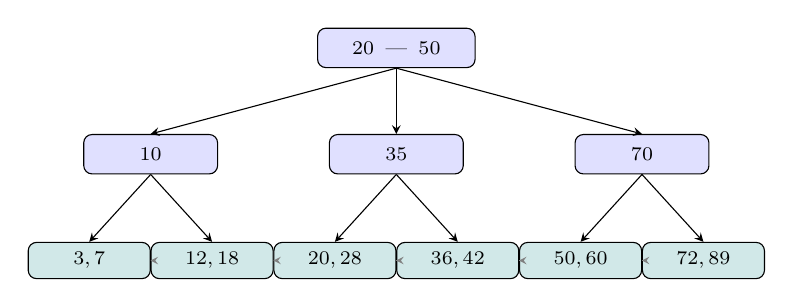
\begin{tikzpicture}[
    x=1.04cm, y=1cm,
    inode/.style={draw, rounded corners=3pt,
                  minimum width=1.7cm, minimum height=0.5cm,
                  font=\scriptsize, fill=blue!12},
    leaf/.style={draw, rounded corners=3pt,
                 minimum width=1.55cm, minimum height=0.46cm,
                 font=\scriptsize, fill=teal!18},
    arr/.style={->, >=stealth, thin},
    chain/.style={->, >=stealth, very thin, dashed, gray}
]
% centres feuilles (unités x) : 0.75 2.25 3.75 5.25 6.75 8.25
% centres L1 : 1.5  4.5  7.5
% racine : 4.5

% Racine
\node[inode, minimum width=2.0cm] (root) at (4.5, 0) {20 \,|\, 50};

% Niveau 1
\node[inode] (n1) at (1.5,  -1.35) {10};
\node[inode] (n2) at (4.5,  -1.35) {35};
\node[inode] (n3) at (7.5,  -1.35) {70};

% Racine → N1
\draw[arr] (root.south) -- (n1.north);
\draw[arr] (root.south) -- (n2.north);
\draw[arr] (root.south) -- (n3.north);

% Feuilles
\node[leaf] (l1) at (0.75, -2.7) {3,\,7};
\node[leaf] (l2) at (2.25, -2.7) {12,\,18};
\node[leaf] (l3) at (3.75, -2.7) {20,\,28};
\node[leaf] (l4) at (5.25, -2.7) {36,\,42};
\node[leaf] (l5) at (6.75, -2.7) {50,\,60};
\node[leaf] (l6) at (8.25, -2.7) {72,\,89};

% N1, N2, N3 → feuilles
\draw[arr] (n1.south) -- (l1.north);
\draw[arr] (n1.south) -- (l2.north);
\draw[arr] (n2.south) -- (l3.north);
\draw[arr] (n2.south) -- (l4.north);
\draw[arr] (n3.south) -- (l5.north);
\draw[arr] (n3.south) -- (l6.north);

% Chaînage horizontal des feuilles
\draw[chain] (l1.east) -- (l2.west);
\draw[chain] (l2.east) -- (l3.west);
\draw[chain] (l3.east) -- (l4.west);
\draw[chain] (l4.east) -- (l5.west);
\draw[chain] (l5.east) -- (l6.west);
\end{tikzpicture}
\end{center}

\vspace{0.1cm}

% ── Blocs de texte — 3 colonnes ─────────────────────────────
\begin{columns}[T]

\column{0.31\textwidth}
\begin{block}{Principe}
\footnotesize
\begin{itemize}
    \item Structure équilibrée d'indexation
    \item Nœuds internes : navigation
    \item Feuilles : clés + pointeurs
    \item Recherche en $\mathcal{O}(\log n)$
\end{itemize}
\end{block}

\column{0.33\textwidth}
\begin{alertblock}{\footnotesize Sans index}
    \centering\scriptsize
    Parcours complet de la table\\
    $\Rightarrow\;\mathcal{O}(n)$ lectures
\end{alertblock}
\vspace{0.15cm}
\begin{exampleblock}{\footnotesize Avec index B+}
    \centering\scriptsize
    Navigation dans l'arbre\\
    $\Rightarrow\;\mathcal{O}(\log n)$ lectures
\end{exampleblock}

\column{0.31\textwidth}
\begin{alertblock}{Observation}
\footnotesize
Réduit fortement le coût des
recherches, mais ralentit les
insertions : l'arbre doit rester
équilibré après chaque écriture.
\end{alertblock}

\end{columns}

\vfill
{\tiny
Sources : Ramakrishnan \& Gehrke, \textit{Database Management Systems} ;
Silberschatz et al., \textit{Database System Concepts}.
}
\end{frame}

\begin{frame}{Index B+ : bénéfices et compromis}

\small

\begin{block}{Temps d'exécution normalisés (base ligne = 100)}
\centering
\tiny Requêtes analytiques typiques :
\texttt{SUM}, \texttt{GROUP BY}, jointures.
\end{block}

\vspace{-0.15cm}

\begin{center}
\begin{tikzpicture}
\begin{axis}[
    width=0.98\textwidth,
    height=0.60\textheight,
    ybar,
    bar width=14pt,
    ymin=0,
    ymax=267,
    ylabel={Temps relatif},
    symbolic x coords={
        Lecture\\3 colonnes,
        Filtrage,
        Jointure
    },
    xtick=data,
    xticklabel style={
        align=center,
        font=\small
    },
    legend style={
        at={(0.5,1.03)},
        anchor=south,
        legend columns=3,
        font=\scriptsize
    },
    nodes near coords,
    nodes near coords style={font=\scriptsize},
    enlarge x limits=0.38,
    grid=major
]

% Sans indexation
\addplot coordinates {
    (Lecture\\3 colonnes,100)
    (Filtrage,100)
    (Jointure,100)
};

% Avec indexation
\addplot coordinates {
    (Lecture\\3 colonnes,100)
    (Filtrage,17)
    (Jointure,23)
};

% Nos performances
\addplot coordinates {
    (Lecture\\3 colonnes,155)
    (Filtrage,126)
    (Jointure,204)
};

\legend{
    Sans indexation,
    Avec indexation,
    Nos performances
}

\end{axis}
\end{tikzpicture}
\end{center}

\vspace{-0.1cm}

{\tiny
Sources :
Abadi et al., \textit{Column-Stores vs. Row-Stores}
(SIGMOD 2008) ;
\textit{The Design and Implementation of Modern
Column-Oriented Database Systems} (2013).
}

\end{frame}



\section{Conclusion}
\subsection{Conclusion}
\begin{frame}
    \frametitle{Résumé}
    \vspace{0.3cm}

    \begin{beamercolorbox}[
        wd=\textwidth,
        rounded=true,
        shadow=true,
        sep=10pt,
        center
    ]{title}
        {\Huge\bfseries Conclusion}
    \end{beamercolorbox}

    \vspace{0.6cm}

    \begin{itemize}
        \item Les bases des Systèmes de Gestion de Base de Données
        \item Différentes optimisations naïve utilisant l'algèbre relationnelle
        \item Certaines optimisations dépendantes des données que notre SGBD possède
        \item Une analyse des résultats obtenus
    \end{itemize}
\end{frame}

\subsection{Nos ressources}
\begin{frame}
    \frametitle{Nos ressources}
    \textbf{Nos ressources:}
    \begin{itemize}
        \item \href{https://drive.google.com/file/d/1KNmuRBf8CV-s-zqdkUEP8iyYlPgFiglb/view?usp=drive_link}{\textit{The Design and Implementation of Modern Column-Oriented Database Systems} \(2013\)}
        \item \href{https://web.stanford.edu/class/cs345d-01/rl/cstore.pdf}{\textit{C-Store: A Column-oriented DBMS} \(2005\)}
        \item \href{https://link.springer.com/content/pdf/10.1007/s41019-020-00149-7.pdf}{\textit{A Survey on Advancing the DBMS Query Optimizer: Cardinality Estimation, Cost Model, and Plan Enumeration} \(2021\)}
        \item \href{https://www.microsoft.com/en-us/research/wp-content/uploads/2024/12/Extensible-Query-Optimizers-in-Practice.pdf}{\textit{Extensible Query Optimizers in Practice} \(2024\)}
        \item \href{http://webdam.inria.fr/Alice/}{\textit{Foundation of Databases} \(1995\)}
    \end{itemize}
\end{frame}

\end{document}
